\section{Casi d'uso} 
\subsection{Attori dei casi d'uso}
\subsubsection{Attori primari}
\begin{figure}[h]
	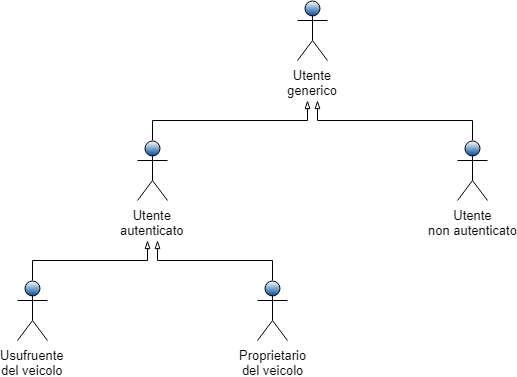
\includegraphics[width=7cm]{res/images/attori_primari.png}
	\centering
	\caption{Gerarchia degli attori primari}
\end{figure}
\begin{description}[style=nextline]
	\item[Utente generico]
	Si riferisce ad un utente generico che entra nell'applicazione.
	\item[Utente non autenticato]
	Si riferisce ad un utente generico che non ha ancora effettuato l'autenticazione nell'applicazione.
	\item[Utente autenticato]
	Si riferisce ad un utente generico che si è autenticato nell'applicazione con la procedura di login.
\end{description}

\subsection{Elenco dei casi d'uso}
In questa sezione vi sono elencati tutti i casi d'uso individuati. Ogni caso d'uso rappresenta uno scenario per uno o più attori, ovviamente applicabile anche ad eventuali attori derivati. Ogni caso d'uso, inoltre, viene descritto tramite diagrammi dei casi d'uso e possiede una precondizione seguita da una postcondizione.
\subsubsection*{Operazioni utenti}
Di seguito sono riportati tutti i casi d'uso che coinvolgono come attore primario l'utente generico, l'utente non autenticato, l'utente autenticato.
\newpage
\begin{figure}[h]
	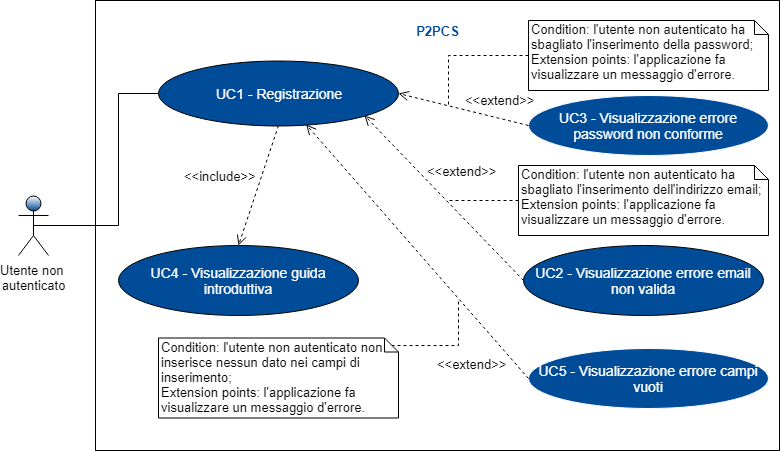
\includegraphics[width=15cm]{res/images/Schemagenerale1.png}
	\centering
	\caption{Schema generale: registrazione ed errori annessi}
\end{figure}
\subsubsection{UC1 - Registrazione}
\begin{figure}
	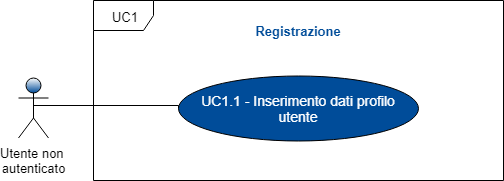
\includegraphics[width=10cm]{res/images/UC1Registrazione.png}
	\centering
	\caption{UC1 - Registrazione}
\end{figure}
\begin{itemize}
	\item \textbf{Attori Primari}: utente non autenticato;
	\item \textbf{Descrizione}: per effettuare il procedimento di registrazione, l'utente deve compilare tutti i campi necessari ovvero nome, cognome, email e password;
	\item \textbf{Scenario principale}: l'applicazione rende disponibili i campi da compilare per la registrazione. Dunque l'utente dovrà inserire tutti i dati necessari, quali:
		\begin{itemize}
			\item Inserimento nome [UC1.1.1];
			\item Inserimento cognome [UC1.1.2];
			\item Inserimento indirizzo email [UC1.1.3];
			\item Inserimento password [UC1.1.4].
		\end{itemize}
	\item \textbf{Precondizione}: l'utente ha inserito correttamente tutti i dati necessari nei campi;
	\item \textbf{Postcondizione}: l'utente viene registrato nell'applicazione;
	\item \textbf{Estensioni}:
		\begin{itemize}
			\item Visualizzazione errore email non valida [UC2];
			\item Visualizzazione errore password non conforme [UC3]. 
		\end{itemize} 
\end{itemize}
\subsubsection{UC1.1 - Inserimento dati profilo utente}
\begin{itemize}
	\item \textbf{Attori Primari}: utente non autenticato;
	\item \textbf{Descrizione}:l'utente compila i campi contenenti i dati relativi al profilo utente;
	\item \textbf{Scenario principale}: l'utente compila tutti i campi del form riguardanti l'account, ovvero:
		\begin{itemize}
			\item l'utente inserisce il proprio nome [UC1.1.1];
			\item l'utente inserisce il proprio cognome [UC1.1.2];
			\item l'utente inserisce l'email da associare all'account [UC1.1.3];
			\item l'utente inserisce la password da associare all'account [UC1.1.4].
		\end{itemize}
	\item \textbf{Precondizione}: l'utente è entrato nell'activity\glosp di registrazione;
	\item \textbf{Postcondizione}: l'utente ha compilato tutti i campi richiesti dalla registrazione.
\end{itemize}
\begin{figure}[h]
	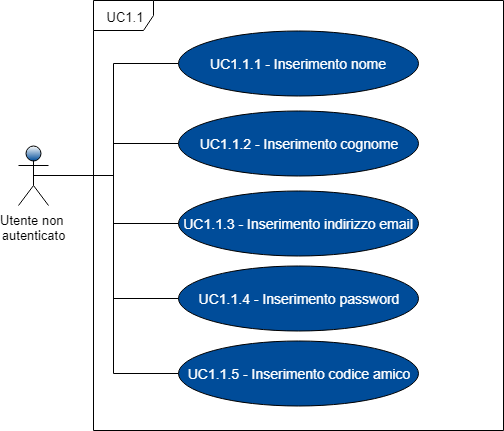
\includegraphics[width=9cm]{res/images/UC1-1Inserimento.png}
	\centering
	\caption{UC1.1 - Inserimento dati profilo utente}
\end{figure}
\newpage
\subsubsection{UC1.1.1 - Inserimento nome}
\begin{itemize}
	\item \textbf{Attori Primari}: utente non autenticato;
	\item \textbf{Descrizione}: al fine di portare a termine il processo di registrazione l'utente deve inserire il proprio nome, campo ritenuto obbligatorio;
	\item \textbf{Scenario principale}: l'utente compila il campo relativo al nome;	
	\item \textbf{Precondizione}: l'applicazione ha reso disponibile il campo per l'inserimento del nome;
	\item \textbf{Postcondizione}: l'utente ha compilato il campo con il proprio nome.	
\end{itemize}
\subsubsection{UC1.1.2 - Inserimento cognome}
\begin{itemize}
	\item \textbf{Attori Primari}: utente non autenticato;
	\item \textbf{Descrizione}: al fine di portare a termine il processo di registrazione l'utente deve inserire il proprio cognome, campo ritenuto obbligatorio;
	\item \textbf{Scenario principale}: l'utente compila il campo relativo al cognome;	
	\item \textbf{Precondizione}: l'applicazione ha reso disponibile il campo per l'inserimento del cognome;
	\item \textbf{Postcondizione}: l'utente ha compilato il campo con il proprio cognome.	
\end{itemize}
\subsubsection{UC1.1.3 - Inserimento indirizzo email}
\begin{itemize}
	\item \textbf{Attori Primari}: utente non autenticato;
	\item \textbf{Descrizione}: al fine di portare a termine il processo di registrazione l'utente deve inserire il proprio indirizzo email, campo ritenuto obbligatorio;
	\item \textbf{Scenario principale}: l'utente compila il campo relativo all'indirizzo email;	
	\item \textbf{Precondizione}: l'applicazione ha reso disponibile il campo per l'inserimento dell'indirizzo email;
	\item \textbf{Postcondizione}: l'utente ha compilato il campo con il proprio indirizzo email.
\end{itemize}
\subsubsection{UC1.1.4 - Inserimento password}
\begin{itemize}
	\item \textbf{Attori Primari}: utente non autenticato;
	\item \textbf{Descrizione}: al fine di portare a termine il processo di registrazione l'utente deve inserire una password, campo ritenuto obbligatorio;
	\item \textbf{Scenario principale}: l'utente compila il campo relativo alla password;	
	\item \textbf{Precondizione}: l'applicazione ha reso disponibile il campo per l'inserimento della password;
	\item \textbf{Postcondizione}: l'utente ha compilato il campo con una password.
\end{itemize}
\subsubsection{UC1.2 - Invio dati}
\begin{itemize}
	\item \textbf{Attori Primari}: utente non autenticato;
	\item \textbf{Descrizione}: l'utente preme il pulsante per la conferma e l'invio dei dati; l'utente verrà rimandato a una nuova activity\glosp che confermerà il successo dell'operazione;
	\item \textbf{Scenario principale}: l'utente preme il pulsante di verifica ed invio dei dati;	
	\item \textbf{Precondizione}: i campi dati necessari per la registrazione sono compilabili. È presente il pulsante per la conferma dei dati;
	\item \textbf{Postcondizione}: l'utente viene rimandato a una nuova activity che conferma il successo dell'operazione e avvisa l'utente di controllare la propria e-mail per confermare il processo di registrazione.
\end{itemize}

\subsubsection{UC2 - Visualizzazione errore email non valida}
\begin{itemize}
	\item \textbf{Attori Primari}: utente non autenticato;
	\item \textbf{Descrizione}: l'utente visualizza un messaggio d'errore in quanto l'email digitata è scorretta;
	\item \textbf{Scenario principale}: l'utente non ancora autenticato tenta di registrarsi inserendo un indirizzo email non valido;
	\item \textbf{Precondizione}: l'utente non autenticato ha sbagliato l'inserimento dell'indirizzo email; 
	\item \textbf{Postcondizione}: l'applicazione fa visualizzare un messaggio d'errore.
\end{itemize}

\subsubsection{UC3 - Visualizzazione errore password non conforme}
\begin{itemize}
	\item \textbf{Attori Primari}: utente non autenticato;
	\item \textbf{Descrizione}: l'utente visualizza un messaggio d'errore in quanto la password digitata non è conforme ai seguenti vincoli:
		\begin{itemize}
			\item ci deve essere almeno una lettera maiuscola;
			\item ci deve essere almeno un carattere speciale;
			\item ci devono essere almeno 8 caratteri;
		\end{itemize}
	\item \textbf{Scenario principale}: l'utente non ancora autenticato tenta di registrarsi inserendo un password errata;
	\item \textbf{Precondizione}: l'utente non autenticato ha sbagliato l'inserimento della password; 
	\item \textbf{Postcondizione}: l'applicazione fa visualizzare un messaggio d'errore.
\end{itemize}

\subsubsection{UC4 - Visualizzazione activity introduttiva}
\begin{itemize}
	\item \textbf{Attori Primari}: utente non autenticato;
	\item \textbf{Descrizione}: l'utente visualizza una guida introduttiva che mostra le funzionalità dell'applicazione nella sue sezioni principali al termine della quale potrà accedere all'activity\glosp di login;
	\item \textbf{Scenario principale}: l'utente accede all'activity introduttiva dell'applicazione e può decidere se visualizzarla o saltarla andando ad effettuare l'accesso;
	\item \textbf{Precondizione}: l'utente si è registrato e può accedere all'activity introduttiva dell'applicazione;
	\item \textbf{Postcondizione}: il sistema fornisce all'utente la possibilità di visualizzare interamente la guida o di saltarla e raggiungere l'activity di login.
\end{itemize}


\begin{figure}[h]
	%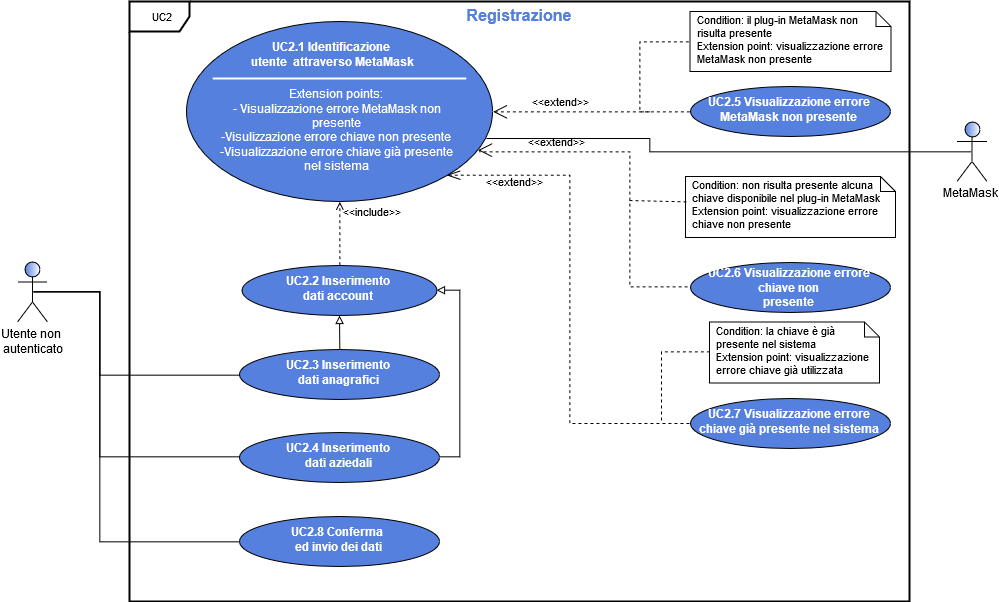
\includegraphics[width=9cm]{res/images/UC2Registrazione.png}
	\centering
	\caption{Schema generale: login ed errori annessi}
\end{figure}
\subsubsection{UC5 - Login}
\begin{itemize}
	\item \textbf{Attori Primari}: utente non autenticato;
	\item \textbf{Descrizione}: per effettuare il procedimento di autenticazione, l'utente deve compilare i campi necessari ovvero e-mail e password;
	\item \textbf{Scenario principale}: l'applicazione rende disponibili i campi da compilare per l'autenticazione. Dunque l'utente dovrà inserire tutti i dati necessari;
	\item \textbf{Precondizione}: l'utente ha inserito correttamente tutti i dati necessari nei campi;
	\item \textbf{Postcondizione}: dopo aver controllato che i campi sono stati compilati correttamente attraverso la piattaforma Movens\glo, l'utente viene autenticato nell'applicazione.
	\item \textbf{Estensioni}:
		\begin{enumerate}
			\item Visualizzazione errore campi vuoti [UC6];
			\item Visualizzazione errore combinazione e-mail e password errata [UC7].
		\end{enumerate}	
\end{itemize}
\begin{figure}[h]
	%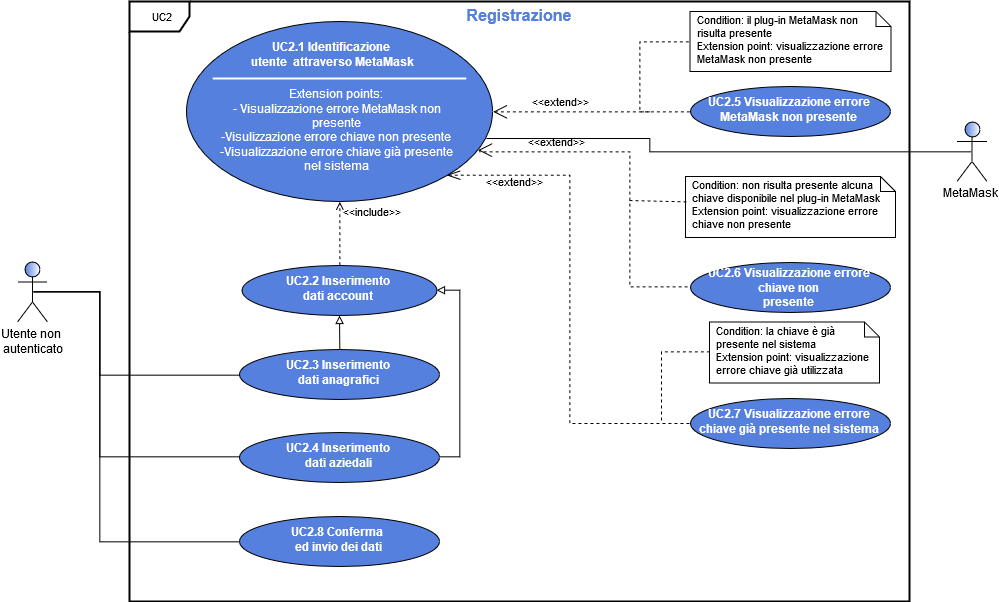
\includegraphics[width=9cm]{res/images/UC2Registrazione.png}
	\centering
	\caption{UC5 - Login}
\end{figure}
\subsubsection{UC5.1 - Compilazione campi per il login}
\begin{figure}[h]
	%\includegraphics[width=9cm]{res/images/UC3-1Login.png}
	\centering
	\caption{UC5.1 - Compilazione campi per il login}
\end{figure}
\begin{itemize}
	\item \textbf{Attori Primari}: utente non autenticato;
	\item \textbf{Descrizione}: l'utente compila i campi richiesti per l'autenticazione;
	\item \textbf{Scenario principale}: l'utente compila i campi necessari all'autenticazione ovvero:
		\begin{itemize}
			\item l'utente inserisce l'email associata al proprio account [UC5.1.1];
			\item l'utente inserisce la password associata la proprio account [UC5.1.2].
		\end{itemize}	
	\item \textbf{Precondizione}: l'utente si trova nell'activity\glosp di autenticazione;
	\item \textbf{Postcondizione}: l'utente ha compilato tutti i campi necessari all'autenticazione.	
\end{itemize}

\subsubsection{UC5.1.1 - Inserimento e-mail}
\begin{itemize}
	\item \textbf{Attori Primari}: utente non autenticato;
	\item \textbf{Descrizione}: al fine di portare a termine il processo di autenticazione l'utente deve inserire l'indirizzo e-mail associato all'account, campo ritenuto obbligatorio;
	\item \textbf{Scenario principale}: l'utente compila il campo relativo all'indirizzo e-mail;	
	\item \textbf{Precondizione}: l'applicazione ha reso disponibile il campo per l'inserimento dell'indirizzo e-mail;
	\item \textbf{Postcondizione}: l'utente ha compilato il campo con l'indirizzo e-mail associato al proprio account.
\end{itemize}

\subsubsection{UC5.1.2 - Inserimento password}
\begin{itemize}
	\item \textbf{Attori Primari}: utente non autenticato;
	\item \textbf{Descrizione}: al fine di portare a termine il processo di autenticazione l'utente deve inserire la password associata al proprio account, campo ritenuto obbligatorio;
	\item \textbf{Scenario principale}: l'utente compila il campo relativo alla password;	
	\item \textbf{Precondizione}: l'applicazione ha reso disponibile il campo per l'inserimento della password;
	\item \textbf{Postcondizione}: l'utente ha compilato il campo con la password associata al proprio account.
\end{itemize}

\subsubsection{UC5.2 - Invio dati}
\begin{itemize}
	\item \textbf{Attori Primari}: utente non autenticato;
	\item \textbf{Descrizione}: l'utente preme il pulsante per la conferma e l'invio dei dati; se e-mail e password risulteranno corrette l'utente verrà autenticato;
	\item \textbf{Scenario principale}: l'utente preme il pulsante di verifica ed invio dei dati;	
	\item \textbf{Precondizione}: i campi dati necessari per l'autenticazione sono compilabili. È presente il pulsante per la conferma dei dati;
	\item \textbf{Postcondizione}: l'utente viene autenticato e rimandato all'activity\glosp per la gestione dei veicoli.
\end{itemize}

\subsubsection{UC6 - Visualizzazione errore campi vuoti}
\begin{itemize}
	\item \textbf{Attori Primari}: utente non autenticato;
	\item \textbf{Descrizione}: l'utente visualizza un messaggio d'errore in quanto non sono stati riempiti i campi di inserimento e-mail e password;
	\item \textbf{Scenario principale}: l'utente non ancora autenticato tenta di accedere non inserendo un indirizzo e-mail e password;	
	\item \textbf{Precondizione}: l'utente non autenticato non inserisce nessun dato nei campi di inserimento;
	\item \textbf{Postcondizione}: l'applicazione fa visualizzare un messaggio d'errore.
\end{itemize}
\subsubsection{UC7 - Visualizzazione errore combinazione e-mail e password errata}
\begin{itemize}
	\item \textbf{Attori Primari}: utente non autenticato;
	\item \textbf{Descrizione}: l'utente visualizza un messaggio d'errore in quanto i campi di inserimento e-mail e password sono stati riempiti in modo errato;
	\item \textbf{Scenario principale}: l'utente non ancora autenticato tenta di accedere inserendo un indirizzo e-mail e password che insieme risultano non validi;	
	\item \textbf{Precondizione}: l'utente non autenticato inserisce i dati che combinati risultano non validi;
	\item \textbf{Postcondizione}: l'applicazione fa visualizzare un messaggio d'errore.
\end{itemize}

\subsubsection{UC8 - Recupero password}
\begin{itemize}
	\item \textbf{Attori Primari}: utente non autenticato;
	\item \textbf{Descrizione}: l'utente non autenticato tenta
	\item \textbf{Scenario principale}: l'utente non ancora autenticato tenta di accedere non inserendo un indirizzo e-mail e password;	
	\item \textbf{Precondizione}: l'utente non autenticato non inserisce nessun dato nei campi di inserimento;
	\item \textbf{Postcondizione}: l'applicazione fa visualizzare un messaggio d'errore.
\end{itemize}

\subsubsection{UC9 - Logout}
\begin{itemize}
	\item \textbf{Attori Primari}:
	utente autenticato;
	\item \textbf{Descrizione}: l'utente dal fragment\glosp Area Personale richiede il logout dall'applicazione;
	\item \textbf{Scenario principale}: l'utente è autenticato nell'applicazione e richiede di effettuare il logout, premendo sull'apposito pulsante;
	\item \textbf{Precondizione}: l'utente ha effettuato il login all'applicazione e richiede di essere disconnesso dall'applicazione;
	\item \textbf{Postcondizione}: l'utente viene disautenticato e rimandato all'activity introduttiva. 
\end{itemize}


 \subsubsection{UC8 - Gestione Veicoli}
  \begin{figure}[H]
 	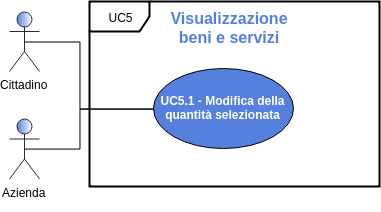
\includegraphics[width=6cm]{res/images/UC5-Generale.png}
 	\centering
 	\caption{UC5 - Gestione Veicoli}
 \end{figure}
 \begin{itemize}
 	\item \textbf{Attori Primari}: utente autenticato;
 	\item \textbf{Descrizione}: l'utente visualizza i propri veicoli. Per ogni veicolo vengono visualizzate le seguenti informazioni:
 	\begin{itemize}
 		\item marca;
 		\item modello;
 		\item anno di immatricolazione;
 		\item rating;
 	\end{itemize}
 	\item \textbf{Precondizione}: l'utente accede al fragment\glosp per la gestione dei veicoli;
 	\item \textbf{Postcondizione}: l'utente visualizza le informazioni relative ai propri veicoli, con le eventuali operazioni disponibili su ognuno di essi.
 \end{itemize}
 \subsubsection{UC5.1 - Aggiunta Veicolo}
 \begin{itemize}
 	\item \textbf{Attori Primari}: utente autenticato;
 	\item \textbf{Descrizione}: l'utente può aggiungere un mezzo di trasporto al proprio parco macchine;
 	\item \textbf{Scenario principale}: l'utente aggiunge un veicolo; l'utente attraverso appositi campi ne deve specificare marca e modello;
 	\item \textbf{Precondizione}: l'utente sta visualizzando un prodotto ed intende modificarne la quantità selezionata;
 	\item \textbf{Postcondizione}: la quantità del prodotto è stata aggiornata al nuovo valore selezionato.
 \end{itemize}
\subsubsection{UC11 - Gestione prenotazione}
 \begin{figure}[h]
	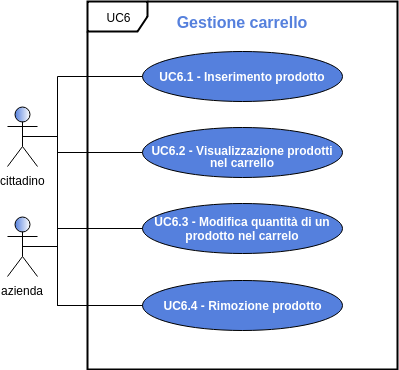
\includegraphics[width=6cm]{res/images/UC6GestioneCarrello.png}
	\centering
	\caption{UC11 - Gestione prenotazione}
\end{figure}
\begin{itemize}
	\item \textbf{Attori Primari}: utente autenticato;
	\item \textbf{Descrizione}: agli utenti autenticati è resa disponibile una maschera che presenta la lista di tutte le sue prenotazioni, dalla quale l'utente può scegliere di effettuare operazioni di gestione su ognuna di esse;
	Per ogni prenotazione presente nella lista saranno visualizzati dei dettagli riassuntivi, che sono:
	\begin{itemize}
		\item \textit{da completare in seguito}.
	\end{itemize}
	\item \textbf{Scenario principale}: l'utente effettua operazioni di gestione di una prenotazione. Esse comprendono:
	\begin{enumerate}[label=\alph*.]
		\item la visualizzazione dei dettagli di una prenotazione [UC11.1];
		\item la modifica di una prenotazione [UC11.2];
		\item la cancellazione di una prenotazione [UC11.3].
	\end{enumerate}
	\item \textbf{Precondizione}: il sistema riconosce l'utente proprietario o usufruente e rende disponibile il servizio di gestione delle prenotazioni;
	\item \textbf{Post-condizione}: l'utente riconosciuto può procedere con le operazioni di gestione rese disponibili.
\end{itemize} 
 \subsubsection{UC11.1 - Visualizzazione dettagli prenotazione}
\begin{itemize}
	\item \textbf{Attori Primari}: utente autenticato;
	\item \textbf{Descrizione}: l'utente visualizza i dettagli della prenotazione scelta dalla maschera di presentazione delle prenotazioni;
	\item \textbf{Scenario principale}:
	\begin{enumerate}[label=\alph*.]
		\item l'utente sta visualizzando i dettagli della prenotazione;
		\item l'utente sceglie di modificare la prenotazione scelta [UC11.2];
		\item l'utente sceglie di eliminare la prenotazione scelta [UC11.3].
	\end{enumerate}
	\item \textbf{Precondizione}: l'utente sta visualizzando i dettagli della prenotazione scelta dalla maschera di presentazione delle prenotazioni;
	\item \textbf{Post-condizione}: l'utente ha visualizzato e/o modificato la prenotazione precedentemente scelta.
\end{itemize}
\begin{comment}

\subsubsection{UC6.2 - Modifica di una prenotazione}
\begin{itemize}
	\item \textbf{Attori Primari}: utente autenticato;
	\item \textbf{Descrizione}: l'utente modifica uno o più dati della prenotazione selezionata;
	\item \textbf{Scenario principale}: l'utente si trova all'interno della pagina di modifica della prenotazione precedentemente selezionata;
	\item \textbf{Precondizione}: l'utente si trova nella pagina di presentazione di tutte le sue prenotazioni e ne ha selezionato una per la modifica, oppure l'utente si trova nella pagina di visualizzazione dettagli prenotazione e sceglie di modificare quest'ultima;
	\item \textbf{Post-condizione}: l'utente ha modificato uno o più dati della prenotazione selezionata.
\end{itemize}

\end{comment}
\subsubsection{UC11.3 - Cancellazione di una prenotazione}
\begin{itemize}
	\item \textbf{Attori Primari}: utente autenticato;
	\item \textbf{Descrizione}: l'utente cancella la prenotazione selezionata;
	\item \textbf{Scenario principale}: l'utente si trova all'interno della pagina di cancellazione della prenotazione precedentemente selezionata. Verrà chiesta conferma all'utente prima di procedere con la cancellazione;
	\item \textbf{Precondizione}: l'utente si trova nella pagina di presentazione di tutte le sue prenotazioni e ne ha selezionato una per la cancellazione, oppure l'utente si trova nella pagina di visualizzazione dettagli prenotazione e sceglie di cancellare quest'ultima;
	\item \textbf{Post-condizione}: l'utente ha confermato o annullato la cancellazione della prenotazione selezionata.
\end{itemize}

\subsubsection{UC12 - Gestione Profilo}
%\begin{figure}[h]
	%\includegraphics[width=10cm]{res/images/UC7-profilepage.png}
	%\centering
	%\caption{UC7 - Gestione Profilo}
%\end{figure}
\begin{itemize}
	\item \textbf{Attori Primari}: utente autenticato;
	\item \textbf{Descrizione}: all'utente è permesso modificare i dati del proprio account oppure eliminarlo;
	\item \textbf{Scenario principale}: 
	\begin{enumerate}[label=\alph*.]
		\item l'utente sceglie di modificare i dati[UC7.1];
		\item l'utente sceglie di eliminare l'account[UC7.3];
	\end{enumerate}
	
	\item \textbf{Precondizione}: l'utente è in possesso di un account all'interno del sistema. Deve quindi essersi registrato e non aver eliminato l'account;
	\item \textbf{Postcondizione}:l'utente ha effettuato l'operazione di modifica dati oppure l'eliminazione dell'account e il processo è stato confermato dal sistema.
	\item \textbf{Estensioni}:
	\begin{enumerate}
	\item visualizzazione di errore sui dati in input[UC7.2]
	\end{enumerate}
\end{itemize} 
\subsubsection{UC7.1 - Modifica dati account}
\begin{itemize}
	\item \textbf{Attori Primari}: utente autenticato;
	\item \textbf{Descrizione}: l'utente ha la possibilità di modificare i propri dati;
	\item \textbf{Scenario principale}:
	\begin{enumerate}
	\item modifica  password[UC7.1.1];
	\item conferma modifica[UC7.1.3].
	\end{enumerate}
	\item \textbf{Inclusioni}:
	\begin{enumerate}
	\item inserimento vecchia password[7.1.2].
	\end{enumerate}
	\item \textbf{Scenari alternativi}:
	\begin{enumerate}
	\item l'utente interrompe la modifica dei dati senza confermare il salvataggio di essi. Il sistema non salverà le modifiche parziali apportate dall'utente me lo riporterà alla schermata di visualizzazione dell'account.
	\end{enumerate}	 
	\item \textbf{Precondizione}: l'utente è in possesso di un account all'interno del sistema. Deve quindi essersi registrato e non aver eliminato l'account;
	\item \textbf{Postcondizione}: il sistema ha memorizzato le modifiche apportate ai dati da parte dell’utente.
\end{itemize}

\subsubsection{UC7.1.1 - Modifica password}
\begin{itemize}
	\item \textbf{Attori Primari}: utente autenticato;
	\item \textbf{Descrizione}: l'utente ha la possibilità di modificare la password inserita in precedenza;
	\item \textbf{Precondizione}: il sistema fornisce una schermata nella quale è possibile inserire la nuova password;
	\item \textbf{Postcondizione}: l'utente ha inserito la nuova password.
\end{itemize}

\subsubsection{UC7.1.2 - Inserimento vecchia password}
\begin{itemize}
	\item \textbf{Attori Primari}: utente autenticato;
	\item \textbf{Descrizione}: l'utente deve inserire la password attuale per poter la aggiornare;
	\item \textbf{Precondizione}: il sistema fornisce una schermata nella quale è possibile inserire la vecchia password;
	\item \textbf{Postcondizione}: l'utente ha inserito la vecchia password.
\end{itemize}

\subsubsection{UC7.1.3 - Modifica patente}
\begin{itemize}
	\item \textbf{Attori Primari}: utente autenticato;
	\item \textbf{Descrizione}: l'utente ha la possibilità di aggiornare la patente inserita in precedenza;
	\item \textbf{Precondizione}: il sistema fornisce una schermata nella quale è possibile inserire la nuova patente;
	\item \textbf{Postcondizione}: l'utente ha inserito la nuova patente.
\end{itemize}

\subsubsection{UC7.1.4 - Conferma modifica dati}
\begin{itemize}
	\item \textbf{Attori Primari}: utente autenticato;
	\item \textbf{Descrizione}: l'utente deve 
	confermare la modifica apportata;
	\item \textbf{Precondizione}: l'utente ha inserito tutti i dati richiesti e desiderati. Si trova dunque davanti ad una schermata con la possibilità di confermare la modifica effettutata;
	\item \textbf{Postcondizione}: l'utente ha confermato di voler rendere effettivo il cambiamento all'interno del sistema.
\end{itemize}

\subsubsection{UC7.2 - Errore nei dati in input}
\begin{itemize}
	\item \textbf{Attori Primari}: utente autenticato;
	\item \textbf{Descrizione}: durante la fase di modifica dei dati, l'utente può aver commesso uno dei seguenti errori:
	\begin{itemize}[label=$-$]
	\item la password inserita in UC7.1.2 non corrisponde con la vecchia password;
	\item la password nuova inserita non è conforme ai vincoli di sicurezza imposti dal sistema;
	\item la nuova patente inserita non è valida.	
	\end{itemize}
	\item \textbf{Precondizione}: l'utente ha effettuato la conferma dei dati inseriti;
	\item \textbf{Postcondizione}: viene notificato all'utente un errore nell'inserimento dei dati. Bisogna specificare l'errore commesso e su quali dati.
\end{itemize}

\subsubsection{UC7.3 - Eliminazione account}
\begin{itemize}
	\item \textbf{Attori Primari}: utente autenticato;
	\item \textbf{Descrizione}: all'utente viene fornita la possibilità di eliminare il proprio account e di conseguenza i propri dati all'interno del sistema.
	\item \textbf{Precondizione}: l'utente è in possesso di un account all'internodel sistema. Deve quindi aver effettuato la registrazione e non avere mai efettuato la procedura di eliminazione account.
	\item \textbf{Postcondizione}: l'utente ha cancellato il proprio account e viene riportato alla schermata iniziale dell'app[UC1].Il sistema non dovrà avere più taccia di tale utente.
\end{itemize}


%Errori UC13






\subsubsection{UC8 - Gestione prodotti in vendita}
\begin{figure}[h]
	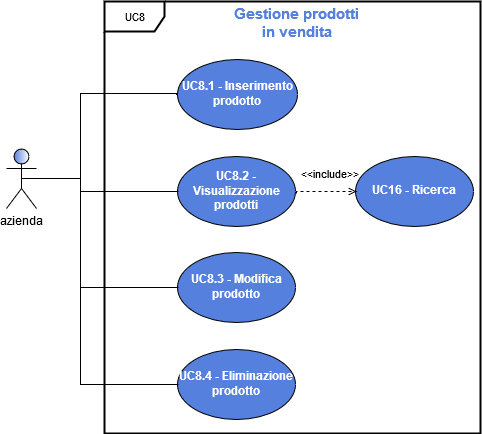
\includegraphics[width=8cm]{res/images/UC8-Generale.png}
	\centering
	\caption{UC8 - Gestione prodotti in vendita}
\end{figure}
\begin{itemize}
	\item \textbf{Attori Primari}: azienda;
	\item \textbf{Descrizione}: le aziende hanno la possibilità di gestire i propri beni in vendita sulla piattaforma;
	\item \textbf{Scenario principale}: l'azienda accede alla pagina per la gestione dei beni/servizi venduti e può:
	\begin{itemize}
		\item inserire un nuovo prodotto da vendere [UC8.1];
		\item visualizzare i propri prodotti attualmente in vendita [UC8.2];
		\item modificare un prodotto già presente nella piattaforma [UC8.3];
		\item rimuovere un prodotto presente [UC8.4].
	\end{itemize}
	\item \textbf{Precondizione}: il sistema ha identificato l'utente come azienda, l'azienda si trova nella pagina per la gestione dei propri beni/servizi;
	\item \textbf{Postcondizione}: il sistema fornisce all'azienda le operazioni che possono essere svolte sui propri beni/servizi.	
\end{itemize}

\subsubsection{UC8.1 - Inserimento prodotto}
\begin{figure}[h]
	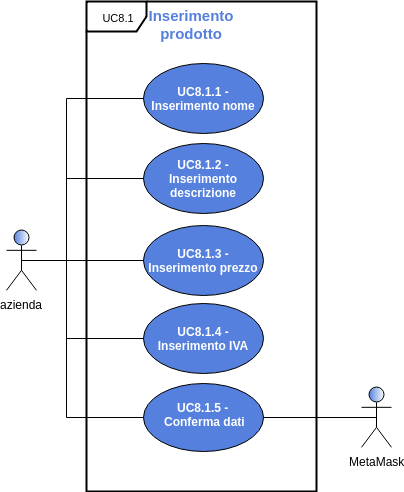
\includegraphics[width=8cm]{res/images/UC8-Inserimento.png}
	\centering
	\caption{UC8.1 - Inserimento prodotto}
\end{figure}
\begin{itemize}
	\item \textbf{Attori Primari}: azienda;
	\item \textbf{Attori Secondari}: MetaMask\glo;
	\item \textbf{Descrizione}: le aziende possono inserire dei nuovi prodotti nella piattaforma;
	\item \textbf{Scenario principale}: l'azienda accede alla pagina per inserire un nuovo prodotto e deve:
	\begin{enumerate}[label=\alph*.]
			\item inserire il nome del bene/servizio [UC8.1.1];
		\item inserire la descrizione del bene/servizio [UC8.1.2];
		\item inserire il prezzo netto unitario del bene/servizio [UC8.1.3];
		\item inserire l'IVA del bene/servizio [UC8.1.4];
		\item confermare i dati inseriti [UC8.1.5].
	\end{enumerate}
	
	\item \textbf{Precondizione}: il sistema ha identificato l'utente come azienda, l'azienda si trova nella pagina di gestione dei beni/servizi;
	\item \textbf{Postcondizione}: l'azienda ha inserito correttamente i dati relativi al nuovo prodotto ed è riuscita ad inserire il nuovo prodotto sulla piattaforma.	
\end{itemize}
\subsubsection{UC8.1.1 - Inserimento nome}
\begin{itemize}
	\item \textbf{Attori Primari}: azienda;
	\item \textbf{Descrizione}: al fine di portare a termine il processo di inserimento di un nuovo prodotto l'azienda deve inserire il nome del prodotto, campo ritenuto obbligatorio;
	\item \textbf{Scenario principale}: l'azienda compila il campo relativo al nome del nuovo prodotto da inserire;
	\item \textbf{Precondizione}: il sistema ha reso disponibile il form per l'inserimento di un nuovo prodotto, in particolare è presente il campo per l'inserimento del nome;
	\item \textbf{Postcondizione}: l'azienda ha compilato il campo relativo al nome del nuovo prodotto da inserire.
\end{itemize}
\subsubsection{UC8.1.2 - Inserimento descrizione}
\begin{itemize}
	\item \textbf{Attori Primari}: azienda;
	\item \textbf{Descrizione}: al fine di portare a termine il processo di inserimento di un nuovo prodotto l'azienda deve inserire la descrizione del prodotto, campo ritenuto obbligatorio;
	\item \textbf{Scenario principale}: l'azienda compila il campo relativo alla descrizione del nuovo prodotto da inserire;
	\item \textbf{Precondizione}: il sistema ha reso disponibile il form per l'inserimento di un nuovo prodotto, in particolare è presente il campo per l'inserimento della descrizione;
	\item \textbf{Postcondizione}: l'azienda ha compilato il campo relativo alla descrizione del nuovo prodotto da inserire.
\end{itemize}
\subsubsection{UC8.1.3 - Inserimento prezzo netto}
\begin{itemize}
	\item \textbf{Attori Primari}: azienda;
	\item \textbf{Descrizione}: al fine di portare a termine il processo di inserimento di un nuovo prodotto l'azienda deve inserire il prezzo netto unitario del prodotto, campo ritenuto obbligatorio;
	\item \textbf{Scenario principale}: l'azienda compila il campo relativo al prezzo del nuovo prodotto da inserire;
	\item \textbf{Precondizione}: il sistema ha reso disponibile il form per l'inserimento di un nuovo prodotto, in particolare è presente il campo per l'inserimento del prezzo;
	\item \textbf{Postcondizione}: l'azienda ha compilato il campo relativo al prezzo del nuovo prodotto da inserire.
\end{itemize}
\subsubsection{UC8.1.4 - Inserimento IVA}
\begin{itemize}
	\item \textbf{Attori Primari}: azienda;
	\item \textbf{Descrizione}: al fine di portare a termine il processo di inserimento di un nuovo prodotto l'azienda deve inserire l'aliquota\glosp IVA che intende applicare al prodotto;
	\item \textbf{Scenario principale}: l'utente compila il campo relativo all'aliquota\glosp IVA del nuovo prodotto da inserire;
	\item \textbf{Precondizione}: il sistema ha reso disponibile il form per l'inserimento di un nuovo prodotto, in particolare è presente il campo per l'inserimento dell'aliquota\glosp IVA;
	\item \textbf{Postcondizione}: l'azienda ha compilato il campo relativo all'aliquota\glosp IVA del nuovo prodotto da inserire.
\end{itemize}
\subsubsection{UC8.1.5 - Conferma dati}
\begin{itemize}
	\item \textbf{Attori Primari}: azienda;
	\item \textbf{Attori Primari}: MetaMask\glo;
	\item \textbf{Descrizione}: al fine di portare a termine il processo di inserimento di un prodotto, l'azienda deve confermare i dati inseriti tramite l'approvazione della transazione, che verrà eseguita attraverso il plug-in MetaMask\glo;
	\item \textbf{Scenario principale}: l'azienda preme il pulsante di conferma dei dati inseriti e valida la transazione con MetaMask\glo;
	\item \textbf{Precondizione}: il sistema ha reso disponibile il form per l'inserimento dei dati riguardanti il nuovo prodotto, l'azienda ha compilato tutti i campi ed ha premuto il pulsante per la conferma.
	\item \textbf{Postcondizione}: il nuovo prodotto è stato inserito nella piattaforma e l'azienda visualizza un messaggio di conferma della riuscita dell'operazione.
\end{itemize}

\subsubsection{UC8.2 - Visualizzazione prodotto}
\begin{itemize}
	\item \textbf{Attori Primari}: azienda;
	\item \textbf{Descrizione}: le aziende possono visualizzare i loro prodotti inseriti nella piattaforma. Per ogni prodotto l'azienda può visualizzarne:
	\begin{itemize}
		\item il nome;
		\item la descrizione;
		\item il prezzo netto unitario;
		\item la percentuale IVA imposta.
	\end{itemize}
	\item \textbf{Scenario principale}: l'azienda accede alla pagina per visualizzare i loro prodotti in vendita;	
	\item \textbf{Inclusione}:
	\begin{itemize}
		\item \textbf{UC16}: Ricerca: nella visualizzazione si può fare una ricerca sui prodotti.
	\end{itemize}
	\item \textbf{Precondizione}: il sistema ha identificato l'utente come azienda, questa ha acceduto alla pagina del proprio account dedicata alla gestione dei prodotti da essa messi in vendita;
	\item \textbf{Postcondizione}: l'azienda ha ottenuto la lista dei propri prodotti assieme alle operazioni eseguibili su di essi.	
\end{itemize}

\subsubsection{UC8.3 - Modifica prodotto}
\begin{figure}[H]
	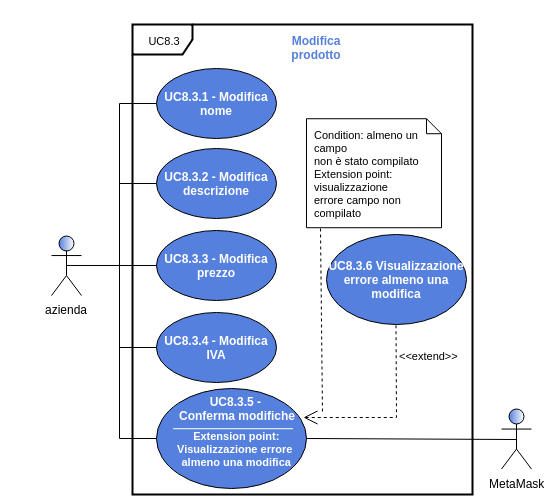
\includegraphics[width=10cm]{res/images/UC8-Modifica.png}
	\centering
	\caption{UC8.3 - Modifica prodotto}
\end{figure}
\begin{itemize}
	\item \textbf{Attori Primari}: azienda;
	\item \textbf{Attori Secondari}: MetaMask\glo;
	\item \textbf{Descrizione}: le aziende possono modificare i loro prodotti inseriti nella piattaforma. In particolare potrà:
	 \begin{itemize}
		\item modificarne il nome [UC8.3.1];
		\item modificarne la descrizione [UC8.3.2];
		\item modificarne il prezzo [UC8.3.3];
		\item modificarne l'IVA [UC8.3.4].
		
	\end{itemize}
	Per ognuno dei campi verrà messo a disposizione il valore attuale ed un campo per inserire il nuovo valore;

	\item \textbf{Scenario principale}: l'azienda accede alla modifica di un prodotto attraverso l'apposito pulsante mostrato assieme alle informazioni riguardanti l'oggetto stesso[UC8.2]. Dunque: 
	\begin{enumerate}[label=\alph*.]
		\item modificare uno o più campi come sopra descritto;
		\item confermare le modifiche [UC8.3.5];
	\end{enumerate}
	Dunque dovrà confermare l'operazione attraverso l'utilizzo di MetaMask\glo.
	
	\item \textbf{Precondizione}: il sistema ha identificato l'utente come azienda, l'azienda si trova sulla pagina di modifica delle informazioni di un particolare prodotto, alla quale è potuta accedere attraverso l'apposito pulsante di modifica del prodotto considerato;
	\item \textbf{Postcondizione}: l'azienda ha modificato le caratteristiche del prodotto. Il sistema visualizza un messaggio per avvisare l'utente del successo dell'operazione.
\end{itemize}

\subsubsection{UC8.3.1 - Modifica nome}
\begin{itemize}
	\item \textbf{Attori Primari}: azienda;
	\item \textbf{Descrizione}: l'azienda inserisce nell'apposito campo il nuovo nome del prodotto;
	\item \textbf{Scenario principale}: l'utente visualizza il vecchio nome con affianco un campo dati per inserire il nuovo nome, ed inserisce il nuovo valore;
	\item \textbf{Precondizione}: il sistema ha reso disponibile il form per la modifica dei dati relativi ad un prodotto messo in vendita dall'azienda;
	\item \textbf{Postcondizione}: l'azienda ha inserito il nuovo nome nel campo dedicato del form.
\end{itemize}

\subsubsection{UC8.3.2 - Modifica descrizione}
\begin{itemize}
	\item \textbf{Attori Primari}: azienda;
	\item \textbf{Descrizione}: l'azienda inserisce nell'apposito campo la nuova descrizione del prodotto;
	\item \textbf{Scenario principale}: l'utente visualizza la vecchia descrizione con affianco un campo dati per inserire la nuova descrizione, ed inserisce il nuovo valore;
	\item \textbf{Precondizione}: il sistema ha reso disponibile il form per la modifica dei dati relativi ad un prodotto messo in vendita dall'azienda;
	\item \textbf{Postcondizione}: l'azienda ha inserito la nuova descrizione nel campo dedicato del form.
\end{itemize}

\subsubsection{UC8.3.3 - Modifica prezzo}
\begin{itemize}
	\item \textbf{Attori Primari}: azienda;
	\item \textbf{Descrizione}: l'azienda inserisce nell'apposito campo il nuovo prezzo del prodotto;
	\item \textbf{Scenario principale}: l'utente visualizza il vecchio prezzo con affianco un campo dati per inserire il nuovo prezzo, ed inserisce il nuovo valore;
	\item \textbf{Precondizione}: il sistema ha reso disponibile il form per la modifica dei dati relativi ad un prodotto messo in vendita dall'azienda;
	\item \textbf{Postcondizione}: l'azienda ha inserito il nuovo prezzo nel campo dedicato del form.
\end{itemize}

\subsubsection{UC8.3.4 - Modifica aliquota IVA}
\begin{itemize}
	\item \textbf{Attori Primari}: azienda;
	\item \textbf{Descrizione}: l'azienda inserisce nell'apposito campo la 
	nuova aliquota IVA imposta al prodotto;
	\item \textbf{Scenario principale}: l'utente visualizza la vecchia aliquota IVA con affianco un campo dati per inserire il nuovo valore, ed compila 
	tale campo;
	\item \textbf{Precondizione}: il sistema ha reso disponibile il form per la modifica dei dati relativi ad un prodotto messo in vendita dall'azienda;
	\item \textbf{Postcondizione}: l'azienda ha inserito la nuova aliquota IVA imposta nel campo dedicato del form.
\end{itemize}

\subsubsection{UC8.3.5 - Conferma modifiche}
\begin{itemize}
	\item \textbf{Attori Primari}: azienda;
	\item \textbf{Attori Primari}: MetaMask\glo;
	\item \textbf{Descrizione}: al fine di portare a termine il processo di modifica dei dati di un bene/servizio, l'utente deve confermare i dati inseriti tramite l'approvazione della transazione, che verrà eseguita attraverso il plug-in MetaMask\glo;
	\item \textbf{Scenario principale}: l'utente preme il pulsante di conferma dei dati inseriti e valida l'operazione con MetaMask\glo;
	\item \textbf{Estensioni}:
	\begin{itemize}
		\item \textbf{UC8.3.6}: l'utente tenta di confermare i dati senza aver compilato almeno uno dei campi.
	\end{itemize}
	\item \textbf{Precondizione}: il sistema ha reso disponibile il form per la modifica dei dati riguardanti un prodotto. L'utente ha compilato almeno un campo ed ha premuto il pulsante per la conferma.
	\item \textbf{Postcondizione}: il prodotto è stato aggiornato con i nuovi dati. Il sistema visualizza un messaggio per avvisare l'utente del fatto che l'operazione è stata eseguita con successo.
\end{itemize}


\subsubsection{UC8.3.6 - Visualizzazione errore almeno una modifica}
\begin{itemize}
	\item \textbf{Attori Primari}: azienda;
	\item \textbf{Descrizione}:
	l'utente visualizza un messaggio di errore relativo al fatto nessuno dei campi per la modifica è stato compilato, e che quindi non è possibile attuare alcuna modifica;
	\item \textbf{Scenario principale}: l'utente tenta di confermare ed inviare le modifiche ai dati senza aver compilato almeno uno dei campi del form;
	\item \textbf{Precondizione}: il sistema permette all'utente di compilare il form per le modifiche. L'utente ha premuto il pulsante di conferma senza aver modificato almeno uno dei campi; 
	\item \textbf{Postcondizione}:
	viene visualizzato un messaggio d'errore per informare l'utente del fatto che, per effettuare una modifica, almeno uno dei dati presenti deve essere stato modificato. È dunque necessario compilare almeno uno dei campi del form.
\end{itemize}

\subsubsection{UC8.4 - Eliminazione prodotto}
\begin{itemize}
	\item \textbf{Attori Primari}: azienda;
	\item \textbf{Attori Primari}: MetaMask\glo;
	\item \textbf{Descrizione}:
	l'azienda elimina uno dei propri beni/servizi presenti sulla piattaforma;
	\item \textbf{Scenario principale}: l'utente clicca sul pulsante di eliminazione prodotto, mostrato assieme alle informazioni riguardanti l'oggetto stesso [UC8.2]. Dunque dovrà confermare l'operazione attraverso l'utilizzo di MetaMask\glo;
	\item \textbf{Inclusione}:
	\begin{itemize}
		\item \textbf{UC8.2}: per poter eliminare i prodotti l'azienda deve prima individuarli nella lista dei propri prodotti.
	\end{itemize}
	\item \textbf{Precondizione}: il sistema ha identificato l'utente come azienda, l'azienda è acceduta alla pagina relativa alla visualizzazione e gestione dei prodotti da essa venduti nella piattaforma;
	\item \textbf{Postcondizione}: l'azienda ha eliminato il prodotto. Il sistema ha visualizzato un messaggio che conferma il successo dell'operazione.
\end{itemize}



\pagebreak
\subsubsection*{Operazioni governative}
Di seguito sono riportati tutti i casi d'uso che coinvolgono come attore primario il governo.

\begin{figure}[H]
	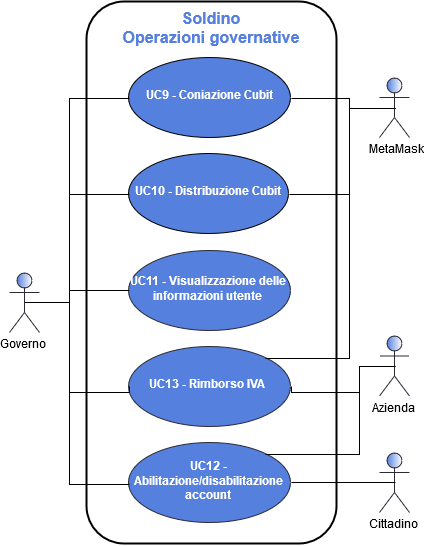
\includegraphics[width=8cm]{res/images/UseCaseGoverno.png}
	\centering
	\caption{Use cases che interessano il governo}
\end{figure}
\subsubsection{UC9 - Coniazione Cubit}
\begin{itemize}
	\item \textbf{Attori Primari}: governo;
	\item \textbf{Attori Secondari}: MetaMask\glo;
	\item \textbf{Descrizione}: viene coniata una quantità definita di Cubit\glo;
	
	\item \textbf{Scenario principale}: il governo ritiene necessario coniare ulteriori Cubit rispetto a quelli attualmente presenti sul mercato. Per fare ciò deve accedere alla pagina dedicata in cui, attraverso un form dovrà:
	 \begin{enumerate}[label=\alph*.]
		\item inserire la quantità $x$ di Cubit da coniare;
		\item confermare tale operazione attraverso l'utilizzo di MetaMask\glo.
	\end{enumerate}
	\item \textbf{Precondizione}: sia $x$ l'ammontare di Cubit che il governo 
	vuole coniare e $n$ l'ammontare di Cubit attualmente in circolo. L'utente 
	governativo ha acceduto alla pagina per la coniazione ed ha compilato e 
	confermato il form;
	\item \textbf{Postcondizione}: i Cubit in circolo sono $x+n$.
\end{itemize}
\subsubsection{UC10 - Distribuzione Cubit}
%non capisco perchè la figura è prima del titolo sul PDF
\begin{figure}[h]
	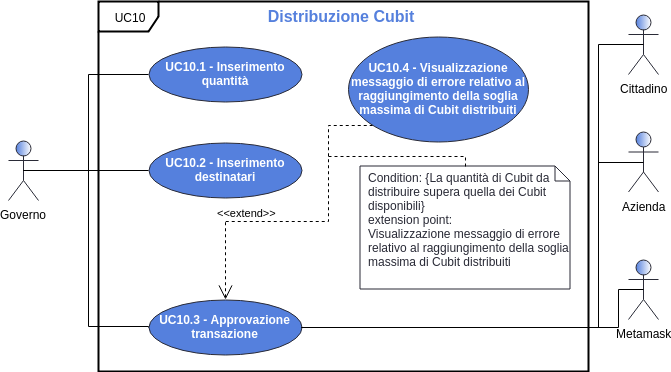
\includegraphics[width=13.5cm]{res/images/UC10Distribuzione.png} %da adattare in larghezza
	\centering
	\caption{UC10 - Distribuzione Cubit}
	
\end{figure}
\begin{itemize}
	\item \textbf{Attori Primari}: governo;
	\item \textbf{Attori Secondari}: MetaMask\glo, cittadino, azienda\glo;
	\item \textbf{Descrizione}: il governo trasferisce una somma di Cubit\glosp sull'account di uno o più  utenti, che siano essi cittadini o aziende;
	\item \textbf{Scenario principale}: il governo deve:
	 \begin{enumerate}[label=\alph*.]
		\item determinare l'ammontare di Cubit pro capite da trasferire [UC10.1];
		\item  selezionare la lista dei destinatari del trasferimento dalla lista degli utenti [UC10.2];
		\item confermare l'operazione [UC10.3].
	\end{enumerate}

	\item \textbf{Precondizione}: il governo accede alla pagina contenente il form per la distribuzione di Cubit agli utenti e compila il suddetto form;
	\item \textbf{Postcondizione}: tali utenti ricevono i Cubit da parte del governo.
\end{itemize}
\subsubsection{UC10.1 - Inserimento quantità}
\begin{itemize}
	\item \textbf{Attori Primari}: governo;
	\item \textbf{Descrizione}: il governo inserisce nell'apposito campo del form la quantità di Cubit\glosp da distribuire, ritenendo la quantità inserita come quantità da inviare ad ogni singolo utente;
	\item \textbf{Scenario principale}: il governo inserisce l'ammontare $x$ di 
	Cubit da inviare;
	\item \textbf{Precondizione}: il governo si trova alla pagina contenente il form per la distribuzione di Cubit agli utenti;
	\item \textbf{Postcondizione}: il campo relativo all'ammontare di Cubit da 
	distribuire pro capite è stato compilato. 
\end{itemize}
\subsubsection{UC10.2 - Inserimento destinatari}
\begin{itemize}
	\item \textbf{Attori Primari}: governo;
	\item \textbf{Attori Secondari}: cittadino, azienda;
	\item \textbf{Descrizione}: il governo inserisce nell'apposito form la lista dei destinatari della quantità di Cubit\glosp precedentemente inserita;
	\item \textbf{Scenario principale}: il governo:
	\begin{enumerate}[label=\alph*.]
		\item visualizza delle liste contenenti i cittadini e le aziende registrate al sito, che sono accompagnati da una checkbox;
		\item l'utente può usare una barra di ricerca per individuare dei particolari utenti;
		\item l'utente governativo spunta le caselle relative agli utenti ai quali intende trasferire la quantità di Cubit precedentemente definita.
	\end{enumerate}
	\item \textbf{Precondizione}: il governo si trova nella pagina atta alla distribuzione dei Cubit e ha selezionato la quantità di Cubit da distribuire;
	\item \textbf{Postcondizione}: il governo ha selezionato uno o più destinatari dalle liste degli utenti, e può procedere con l'approvazione della transazione.
\end{itemize}
\subsubsection{UC10.3 - Approvazione transazione}
\begin{itemize}
	\item \textbf{Attori Primari}: governo;
	\item \textbf{Attori Secondari}: MetaMask\glo, cittadino, azienda\glo;
	\item \textbf{Descrizione}: il governo decide se approvare o rifiutare la transazione;
	\item \textbf{Scenario principale}: il governo ha specificato la somma 
	$x$ di Cubit\glosp da distribuire ad ognuno degli $y$ destinatari;
	\item \textbf{Estensioni}:
	\begin{itemize}
		\item \textbf{UC10.4}: verrà mostrato un messaggio di errore nel caso 
		l'ammontare totale $x\cdot y$ superi la quantità di Cubit disponibili 
		alla distribuzione.
	\end{itemize}
	\item \textbf{Precondizione}: è necessario aver selezionato una lista di destinatari ed una quantità da distribuire ad ogni singolo utente;
	\item \textbf{Postcondizione}: ogni utente riceverà nel proprio wallet\glosp la quantità di Cubit trasferita dal governo.
\end{itemize}
\subsubsection{UC10.4 - Visualizzazione messaggio di errore relativo al raggiungimento della soglia massima di Cubit distribuiti}
\begin{itemize}
	\item \textbf{Attori Primari}: governo;
	\item \textbf{Descrizione}: il governo riceve un messaggio di errore relativo al fatto che ha selezionato una quantità di Cubit\glosp superiore a quella disponibile alla distribuzione;
	\item \textbf{Scenario principale}: il governo clicca sull'apposito pulsante per confermare la transazione di distribuzione, ma non ha sufficienti fondi per completare tale operazione;
	\item \textbf{Precondizione}: il governo deve aver inserito una quantità di Cubit superiore a quella disponibile e cerca di effettuare la transazione;
	\item \textbf{Postcondizione}: viene visualizzato un messaggio d'errore per informare l'utente del fatto che attualmente non dispone dei fondi necessari per effettuare l'operazione di distribuzione.
	
\end{itemize} 

 \subsubsection{UC11 - Visualizzazione delle informazioni utente}
 \begin{figure}[h]
 	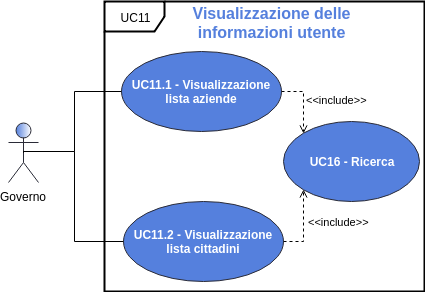
\includegraphics[width=7cm]{res/images/UC11-Generale.png}
 	\centering
 	\caption{UC11 - Visualizzazione delle informazioni utente}
 	
 \end{figure}
 \begin{itemize}
 	\item \textbf{Attori Primari}: governo;
 	\item \textbf{Descrizione}: il governo può accedere alle informazioni riguardanti:
 	\begin{itemize}
 		\item le aziende registrate alla piattaforma;
 		\item i cittadini registrati alla piattaforma.

 	\end{itemize}
 	\item \textbf{Scenario principale}: il governo accede alle informazioni riguardanti gli utenti della piattaforma ed alle eventuali relative operazioni disponibili;

 	\item \textbf{Precondizione}: il sistema riconosce che l'utente è autenticato con privilegi governativi e mostra le pagine utili alla ricerca di informazioni sugli utenti;
 	
 	\item \textbf{Postcondizione}: il governo ottiene dal sistema le liste degli utenti con le eventuali operazioni disponibili.
 \end{itemize}

\subsubsection{UC11.1 - Visualizzazione lista aziende registrate}

 \begin{itemize}
	\item \textbf{Attori Primari}: governo;
	\item \textbf{Descrizione}: il governo visualizza la lista delle aziende registrate alla piattaforma. Per ogni azienda sono rese disponibili le seguenti informazioni:
	\begin{itemize}
		\item chiave\glosp Ethereum\glo;
		\item nome (ragione sociale);
		\item partita IVA;
		\item indirizzo di residenza (sede dell'azienda);
		\item lo stato di "abilitato" o "disabilitato";
		\item indirizzo email;
		\item lo stato del pagamento del saldo IVA, ovvero può controllare se l'azienda risulta:
		\begin{itemize}
			\item \textbf{insolvente}: non ha ancora provveduto alla liquidazione IVA di almeno uno dei trimestri precedenti entro i termini fissati;
			\item \textbf{in fase di pagamento}: l'azienda deve ancora effettuare il versamento IVA riguardante l'ultimo trimestre, ed il termine del pagamento non è ancora scaduto. Nei trimestri antecedenti la situazione risulta "regolare";
			\item \textbf{in dilazione}: in caso l'azienda abbia richiesto il pagamento dilazionato del saldo IVA a debito ed il termine della dilazione non è ancora scaduto;
			\item \textbf{regolare}: l'azienda ha provveduto al pagamento del saldo IVA a debito del trimestre precedente oppure ha ricevuto il rimborso nel caso in cui sia risultata "In attesa di rimborso" nel trimestre precedente;
			\item \textbf{in attesa di rimborso}: nel trimestre precedente il saldo IVA è risultato a credito, e non è ancora stato effettuato il rimborso da parte del governo;
		\end{itemize}
	L'azienda può ricadere in uno solo tra i casi sopra descritti. Lo stato di insolvenza di un trimestre precedente ha la predominanza sugli stati dei trimestri successivi ad esso;
		\item l'importo del saldo IVA.
	\end{itemize}
	
	\item \textbf{Scenario principale}: il governo richiede la lista delle aziende registrate;
	\item \textbf{Inclusioni}:
	\begin{itemize}
		\item \textbf{UC16}: l'utente può filtrare i risultati visualizzati inserendo una parola chiave.
	\end{itemize}
	\item \textbf{Precondizione}: il sistema riconosce che l'utente è autenticato con privilegi governativi ed ha richiesto di ottenere la lista di tutte aziende;
	\item \textbf{Postcondizione}: il governo ottiene dal sistema la lista delle aziende registrate, con associate le operazioni che può effettuare su di esse.
\end{itemize}

\subsubsection{UC11.1.1 - Visualizzazione filtrata lista aziende registrate}
\begin{figure}[H]
	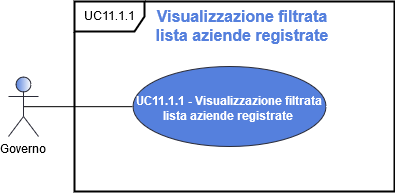
\includegraphics[width=7cm]{res/images/UC11-VisualizzazioneFiltrata.png}
	\centering
	\caption{UC11 - Visualizzazione filtrata lista aziende registrate}
\end{figure}
\begin{itemize}
	\item \textbf{Attori Primari}: governo;
	\item \textbf{Descrizione}: il governo visualizza la lista delle aziende registrate alla piattaforma, filtrate secondo il valore del campo \texttt{stato del pagamento del saldo IVA}. I possibili valori per filtrare i risultati per tale campo sono i seguenti:
	\begin{itemize}
		\item insolvente;
		\item in fase di pagamento;
		\item in dilazione
		\item regolare;
		\item in attesa di rimborso.
	\end{itemize}
	
	\item \textbf{Scenario principale}: il governo filtra le aziende visualizzate secondo il valore del campo \texttt{stato del pagamento del saldo IVA}. Seleziona tale valore servendosi dell'apposito menù a tendina;
	\item \textbf{Precondizione}: l'utente governativo ha eseguito l'accesso alla pagina dedicata alla visualizzazione delle aziende registrate, ed ha selezionato un'opzione per filtrare le aziende;
	\item \textbf{Postcondizione}: il governo ottiene dal sistema la lista delle aziende registrate, filtrate a seconda del valore del campo \texttt{stato del pagamento del saldo IVA} selezionato.
\end{itemize}


\subsubsection{UC11.2 - Visualizzazione lista cittadini}
\begin{itemize}
	\item \textbf{Attori Primari}: governo;
	\item \textbf{Descrizione}: il governo ottiene la lista dei cittadini. Per ognuno di essi può visualizzare:
	\begin{itemize}
		\item la chiave\glosp Ethereum\glo;
		\item il nome;
		\item il cognome;
		\item l'indirizzo di residenza;
		\item indirizzo email.
	\end{itemize}
	\item \textbf{Scenario principale}: il governo richiede la lista dei cittadini. Per ognuno di essi visualizza le rispettive informazioni;
	\item \textbf{Inclusioni}:
	\begin{itemize}
		\item \textbf{UC16}: l'utente può filtrare i risultati visualizzati inserendo una parola chiave.
	\end{itemize}
	\item \textbf{Precondizione}: il sistema riconosce che l'utente è autenticato con privilegi governativi ed ha richiesto di ottenere la lista di tutti i cittadini;
	\item \textbf{Postcondizione}: il governo ottiene dal sistema la lista dei cittadini, con associate le operazioni che può effettuare su di essi.
\end{itemize}



\subsubsection{UC12 - Abilitazione/disabilitazione account}
\begin{figure}[h]
	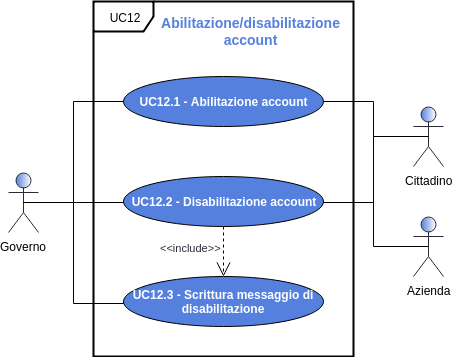
\includegraphics[width=8cm]{res/images/UC12-Generale.png}
	\centering
	\caption{UC12 - Abilitazione/disabilitazione account}
\end{figure}
\begin{itemize}
	\item \textbf{Attori Primari}:
	governo;
	\item \textbf{Attori Secondari}:
	azienda, cittadino;
	\item \textbf{Descrizione}: il governo può gestire gli account degli utenti registrati alla piattaforma, in particolare può:
	\begin{itemize}
		\item abilitare un account;
		\item disabilitare un account, lasciando un messaggio relativo alla causa di tale provvedimento.
	\end{itemize}
	\item \textbf{Scenario principale}: il governo visualizza la lista degli utenti, aziende [UC11.1] o cittadini [UC11.2]. Per ognuna di esse ha la possibilità di abilitare l'account o disabilitarlo premendo l'apposito pulsante;
	\item \textbf{Precondizione}: l'utente governativo sta visualizzando una lista di utenti registrati al sistema, e può quindi accedere al pulsante per l'abilitazione o disabilitazione dell'account di un cittadino;
	\item \textbf{Postcondizione}: l'account dell'utente selezionato è stato abilitato o disabilitato. Nel caso sia stato disabilitato, durante i prossimi tentativi di autenticazione, tale utente riceverà l'errore di "account disabilitato" [UC3.3].
\end{itemize} 

\subsubsection{UC12.1 - Abilitazione account}
\begin{itemize}
	\item \textbf{Attori Primari}:
	governo;
	\item \textbf{Attori Secondari}:
	azienda, cittadino;
	\item \textbf{Descrizione}: il governo può abilitare l'account di un utente;
	\item \textbf{Scenario principale}: il governo visualizza la lista degli utenti, aziende [UC11.1] o cittadini [UC11.2]. Per ogni utente il cui stato dell'account risulta "disabilitato", può effettuare l'abilitazione premendo sul pulsante dedicato;

	\item \textbf{Precondizione}: l'utente governativo sta visualizzando una lista di utenti registrati al sistema, preme il pulsante di abilitazione dell'account relativo ad un utente il quale stato dell'account risulta "disabilitato";
	\item \textbf{Postcondizione}: lo stato  dell'account utente sopra menzionato risulta "abilitato".
\end{itemize} 


\subsubsection{UC12.2 - Disabilitazione account}
\begin{itemize}
	\item \textbf{Attori Primari}:
	governo;
	\item \textbf{Attori Secondari}:
	azienda, cittadino;
	\item \textbf{Descrizione}: il governo può disabilitare l'account di un utente;
	\item \textbf{Scenario principale}: il governo visualizza la lista degli utenti, aziende [UC11.1] o cittadini [UC11.2]. Per ogni utente il cui stato dell'account risulta "abilitato", può effettuare la disabilitazione premendo sul pulsante dedicato;
	\item \textbf{Inclusioni}: 
	\begin{itemize}
		\item \textbf{UC12.3}: durante la disabilitazione l'utente governativo è richiesto di inserire un messaggio personalizzato per spiegare all'utente il motivo della disabilitazione dell'account.
	\end{itemize}
	\item \textbf{Precondizione}: l'utente governativo sta visualizzando una lista di utenti registrati al sistema, preme il pulsante di disabilitazione dell'account relativo ad un utente il quale stato dell'account risulta "abilitato";
	\item \textbf{Postcondizione}: lo stato  dell'account utente sopra menzionato risulta "disabilitato". Durante i prossimi tentativi di autenticazione, tale utente riceverà l'errore di "account disabilitato" [UC3.3].
\end{itemize} 

\subsubsection{UC12.3 - Scrittura messaggio di disabilitazione}
\begin{itemize}
	\item \textbf{Attori Primari}:
	governo;
	\item \textbf{Attori Secondari}:
	azienda, cittadino;
	\item \textbf{Descrizione}: il governo può inserire un messaggio personalizzato all'utente al quale sta disabilitando l'account riferendo la causa di tale disabilitazione;
	\item \textbf{Scenario principale}: il governo visualizza una lista di utenti registrati [UC11]:
	\begin{enumerate}[label=\alph*.]
		\item l'utente governativo disabilita l'account di un utente il cui stato dell'account risulta "abilitato" [UC12.2];
		\item il sistema propone una casella di testo nella quale l'utente governativo può inserire la causa della disabilitazione dell'account;
		\item l'utente governativo conferma e salva tale messaggio. Durante i prossimi tentativi di autenticazione, l'utente al quale è stato disabilitato l'account, riceverà l'errore di "account disabilitato" [UC3.3].
	\end{enumerate}
	 
	\item \textbf{Precondizione}: l'utente governativo ha richiesto la disabilitazione di un account utente premendo sull'apposito pulsante, il sistema visualizza la casella di testo per inserire il messaggio di errore contenente la causa di tale azione;
	\item \textbf{Postcondizione}: l'utente governativo ha inserito un messaggio contenente la causa della disabilitazione dell'account ed ha salvato e confermato tale messaggio.
\end{itemize}


\subsubsection{UC13 - Rimborso IVA}
\begin{itemize}
	\item \textbf{Attori Primari}:
	governo;
	\item \textbf{Attori Secondari}:
	azienda, MetaMask\glo;
	\item \textbf{Descrizione}: il governo effettua il rimborso IVA ad un'azienda che risulta in stato di credito al momento del saldo trimestrale;
	\item \textbf{Scenario principale}: dopo aver visualizzato lo stato IVA di un'azienda [UC11.1] il governo decide di effettuare il rimborso cliccando sul pulsante dedicato. Dovrà confermare la transazione attraverso il plugin MetaMask\glo;
	\item \textbf{Inclusioni}: 
	\begin{itemize}
		\item \textbf{UC11.2}: l'utente per poter accedere al pulsante per il rimborso dell'azienda deve visualizzare la lista delle aziende verificate.
	\end{itemize}
	\item \textbf{Precondizione}: il sistema ha mostrato la lista delle aziende già verificate, con il relativo stato IVA. L'utente ha premuto il pulsante per il rimborso e confermato l'operazione;
	\item \textbf{Postcondizione}: il sistema avvisa l'utente che l'operazione è avvenuta con successo. Il rimborso è stato versato all'azienda.
\end{itemize} 

\subsubsection*{Operazioni di gestione degli ordini e delle fatture}
Di seguito sono riportate tutti i casi d'uso che coinvolgono la gestione degli ordine e delle fatture.

\begin{figure}[H]
	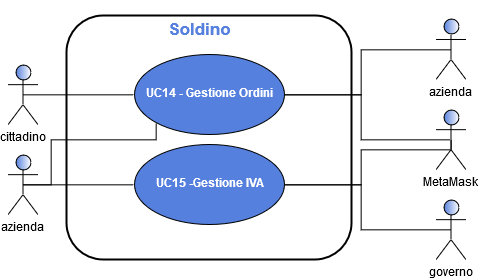
\includegraphics[width=8cm]{res/images/UseCaseFinali.png}
	\centering
	\caption{Use Cases riguardanti la gestione degli ordini e delle fatture}
\end{figure}
\subsubsection{UC14 - Gestione ordini}
\begin{figure}[h]
	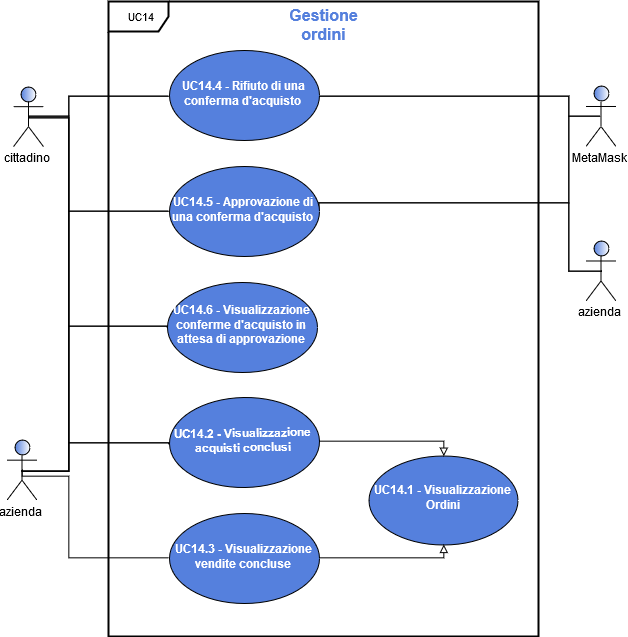
\includegraphics[width=10cm]{res/images/UC14-GestioneOrdini.png}
	\centering
	\caption{UC14 - Gestione ordini}
\end{figure}
\begin{itemize}
	\item \textbf{Attori Primari}: azienda, cittadino;
		\item \textbf{Attori Secondari}: azienda, MetaMask\glo;
	\item \textbf{Descrizione}: agli utenti sono messe a disposizione diverse operazione per visualizzare e gestire gli ordini;
	\item \textbf{Scenario principale}: l'utente visualizza e svolge alcune operazioni per gestire gli ordini nei quali è partecipe;
	\item \textbf{Precondizione}: il sistema ha riconosciuto l'utente autenticato come azienda o cittadino e mette a disposizione tutte le pagine necessarie alla visualizzazione e gestione degli ordini;
	\item \textbf{Postcondizione}: l'utente ha visualizzato e/o gestito i propri ordini.
\end{itemize} 
\subsubsection{UC14.1 - Visualizzazione ordini}
\begin{itemize}
	\item \textbf{Attori Primari}: azienda, cittadino;
	\item \textbf{Descrizione}: alle aziende ed ai cittadini sono messe a disposizione diverse operazioni per visualizzare e gestire gli ordini all'interno della piattaforma. Essi comprendono acquisti e vendite (queste solo per le aziende). \`E reso possibile avere un elenco dettagliato di tutti gli ordini, in particolare per ognuno di essi è possibile la visualizzazione:
	\begin{itemize}
		\item della data dell'ordine;
		\item del numero dell'ordine;
		\item dei prodotti inclusi nell'ordine [UC5];
		\item totale IVA;
		\item totale lordo\glo;
		\item indirizzo di spedizione.
	\end{itemize}
	\item \textbf{Scenario principale}: l'utente visualizza i dati relativi ad un ordine;
	\item \textbf{Specializzazioni}:
	\begin{itemize}
		\item \textbf{UC14.2}: visualizzazione acquisti conclusi.
		\item \textbf{UC14.2}: visualizzazione vendite concluse.
	\end{itemize}
	\item \textbf{Precondizione}: il sistema ha riconosciuto l'utente autenticato come azienda o cittadino e mette a disposizione tutte le pagine necessarie alla visualizzazione e gestione degli ordini;
	\item \textbf{Postcondizione}: l'utente ha visualizzato l'elenco dei propri ordini.
\end{itemize} 



\subsubsection{UC14.2 - Visualizzazione acquisti conclusi}
\begin{itemize}
	\item \textbf{Attori Primari}: cittadino, azienda;
	\item \textbf{Descrizione}: l'azienda ha la possibilità di visualizzare gli acquisti conclusi, ovvero effettuati ed approvati. Oltre ai dati relativi all'ordine sono visualizzate le seguenti informazioni:
	\begin{itemize}
		\item data dell'approvazione dell'ordine;
		\item nome dell'azienda-venditrice;
		\item partita IVA dell'azienda venditrice.
	\end{itemize}
	\item \textbf{Scenario principale}: l'utente visualizza la lista degli acquisti conclusi. 
	\item \textbf{Precondizione}: il sistema ha riconosciuto l’utente autenticato come azienda o cittadino e
	mette a disposizione la pagina di visualizzazione degli acquisti;
	\item \textbf{Postcondizione}: l'utente visualizza la lista degli acquisti conclusi.
\end{itemize}

\subsubsection{UC14.3 - Visualizzazione vendite concluse}
\begin{itemize}
	\item \textbf{Attori Primari}: azienda;
	\item \textbf{Descrizione}: l'azienda ha la possibilità di visualizzare le vendite effettuate ed approvate. Oltre ai dati relative all'ordine sono visualizzare le seguenti informazioni:
		\begin{itemize}
		\item data dell'approvazione;
		\item informazioni riguardanti il cliente:
		\begin{itemize}
			\item nel caso il cliente sia un \textbf{cittadino}:
			\begin{itemize}
				
				\item nome utente;
				\item cognome utente.
			\end{itemize}
			\item nel caso il cliente sia un'\textbf{azienda}:
			\begin{itemize}
				
				\item nome azienda-cliente;
				\item partita IVA dell'azienda-cliente.
			\end{itemize}
		\end{itemize}
		
	\end{itemize}
	\item \textbf{Scenario principale}:  l'utente visualizza le vendite concluse, con alcuni dati relativi al cliente; 
	\item \textbf{Precondizione}: il sistema ha riconosciuto l'utente autenticato come azienda e questo si trova nella pagina dedicata alla visualizzazione delle vendite concluse;
	\item \textbf{Postcondizione}: l'utente visualizza la lista delle vendite concluse.
\end{itemize}


\subsubsection{UC14.4 - Rifiuto di una conferma d'acquisto}
\begin{itemize}
	\item \textbf{Attori Primari}: azienda, cittadino;
	\item \textbf{Attori Secondari}: MetaMask\glo, azienda;
	\item \textbf{Descrizione}: le aziende ed i cittadini possono rifiutare una conferma d'acquisto\glo, ad esempio se notano che i dati inviatogli non corrispondono all'ordine effettuato o le aliquote IVA imposte risultano errate. Per effettuare l'operazione verrà utilizzato MetaMask\glo;
	\item \textbf{Scenario principale}: l'utente visualizza una conferma d'acquisto\glosp che necessita di approvazione e decide di rifiutarla;

	\item \textbf{Precondizione}: il sistema ha riconosciuto l'utente autenticato come cittadino o azienda ed ha mostrato la lista delle proposte d'acquisto\glosp che necessitano di conferma;
	\item \textbf{Postcondizione}: l'azienda ha rifiutato la proposta 
	d'acquisto\glo. La proposta non sarà più presente nella lista di attesa per 
	la conferma. Il sistema ritorna l'ammontare trattenuto per l'ordine 
	all'acquirente.
\end{itemize}
\subsubsection{UC14.5 - Approvazione di una conferma di acquisto}
\begin{itemize}
	\item \textbf{Attori Primari}: azienda, cittadino;
	\item \textbf{Attori Secondari}: MetaMask\glo, azienda;
	\item \textbf{Descrizione}: l'azienda accetta la proposta d'acquisto\glosp ricevuta;
	\item \textbf{Scenario principale}: l'azienda/cittadino decide di approvare una proposta d'acquisto\glosp da parte di un venditore;
	\item \textbf{Scenario alternativo}: l'azienda/cittadino non ha né confermato né approvato la conferma d'acquisto entro la data ultima per l'approvazione;

	\item \textbf{Precondizione}: 
	\begin{enumerate}[label=\alph*.]
		\item il sistema ha riconosciuto l'utente autenticato come azienda o cittadino, e questo ha premuto il bottone per l'approvare una richiesta d'acquisto;
		\item è stata superata la data ultima per il rifiuto della conferma d'ordine\glo.
	\end{enumerate}
	\item \textbf{Postcondizione}: il suddetto ordine risulta approvato. Il meccanismo di escrow\glosp implementato nel sistema rende disponibile la fattura dell'ordine nella pagina dedicata dell'account del cliente. Inoltre l'ammontare relativo all'ordine attualmente trattenuto dal sistema viene versato all'azienda-venditrice.
\end{itemize}


\subsubsection{UC14.6 - Visualizzazione conferme d'acquisto in attesa di 
approvazione}
\begin{itemize}
	\item \textbf{Attori Primari}: azienda, cittadino;
	\item \textbf{Descrizione}: l'azienda/cittadino può visualizzare le conferme d'acquisto\glosp che necessitano di approvazione. Esse sono relative agli acquisti che ha effettuato ma non ancora approvato. Le conferme d'acquisto permettono di visualizzare gli stessi dati relativi ad un ordine, ma ogni prodotto visualizzato ha i seguenti dati aggiuntivi:
	\begin{itemize}
		\item prezzo netto del prodotto acquistato;	
		\item aliquota IVA applicata al prodotto.
	\end{itemize}
	\item \textbf{Scenario principale}: l'utente visualizza la lista delle 
	conferme d'acquisto\glosp che necessitano di conferma. Per ognuna di esse 
	ha la possibilità di confermare la proposta [UC14.5] o di rifiutarla 
	[UC14.4];

	\item \textbf{Precondizione}: il sistema ha riconosciuto l'utente autenticato come azienda o cittadino, e questo si trova nella pagina dedicata alla visualizzazione delle conferme d'acquisto\glosp che necessitano di approvazione;
	\item \textbf{Postcondizione}: l'utente visualizza la lista delle conferme d'ordine\glosp che necessitano di approvazione.
\end{itemize}






\subsubsection{UC15 - Gestione transazioni ed IVA}
\begin{figure}[H]
	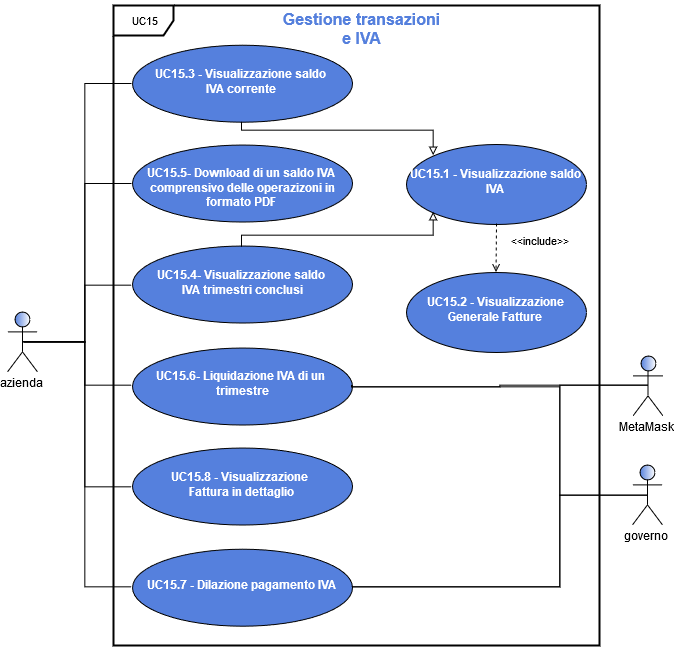
\includegraphics[width=12cm]{res/images/UC15-OK.png}
	\centering
	\caption{UC15 - Gestione transazioni ed IVA}
\end{figure}
\begin{itemize}
	\item \textbf{Attori Primari}: azienda;
	\item \textbf{Descrizione}: alle aziende sono messe a disposizione diverse operazioni per gestire le transazioni e l'IVA:
	\begin{itemize}
		\item può visualizzare i saldi IVA di un periodo, comprendendo la visualizzazione di tutte le transazioni, rappresentate dalle rispettive fatture, e del saldo finale [15.3 \& 15.4];
		\item per ogni fattura è disponibile la visualizzazione dettagliata [15.8];
		\item può scaricare le informazioni riguardanti un trimestre come sopra descritto sotto forma di documento PDF [15.5]; 
		\item in caso il saldo di un semestre risulti negativo (situazione di debito), l'azienda può procedere ad effettuare il versamento al governo [15.6] o può dilazionarlo\glosp [15.7].
	\end{itemize}
	\item \textbf{Scenario principale}: l'utente visualizza e svolge alcune operazioni per gestire l'IVA, gli ordini e le fatture;
	\item \textbf{Precondizione}: il sistema ha riconosciuto l'utente autenticato come azienda, e mette a disposizione tutte le pagine necessarie alla visualizzazione e gestione delle fatture e dell'IVA;
	\item \textbf{Postcondizione}: l'azienda ha visualizzato e/o svolto delle operazioni riguardanti fatture ed IVA.
\end{itemize} 
\subsubsection{UC15.1 - Visualizzazione saldo IVA}
\begin{itemize}
	\item \textbf{Attori Primari}: azienda;
	\item \textbf{Descrizione}: l'azienda può visualizzare il saldo IVA relativo ad un trimestre. In particolare può visualizzare il saldo:
	\begin{itemize}
		\item del trimestre corrente [15.3];
		\item di un trimestre concluso [15.4].
	\end{itemize}
	Il saldo conterrà tutte le fatture relative agli acquisti e le vendite che hanno determinato il suo valore, oltre al valore stesso;
	\item \textbf{Scenario principale}: l'utente visualizza il saldo relativo ad un trimestre. In particolare:
	\begin{enumerate}[label=\alph*.]
		\item seleziona da un menù a tendina uno dei trimestri disponibili;
		\item del trimestre scelto viene visualizzata la relativa lista delle fatture riguardanti gli ordini;
	\end{enumerate}
	\item \textbf{Inclusioni}: 
	\begin{itemize}
		\item \textbf{UC15.2}: visualizzazione generale delle fatture, ovvero il mostrare la lista delle fatture nel saldo.
	\end{itemize}
	\item \textbf{Specializzazioni}: 
	\begin{itemize}
		\item \textbf{UC15.3}: visualizzazione saldo IVA corrente;
		\item \textbf{UC15.4}:  visualizzazione saldo IVA di un trimestre concluso.
	\end{itemize}
	\item \textbf{Precondizione}: il sistema ha riconosciuto l'utente autenticato come azienda, e mette a disposizione le pagine per visualizzazione dei saldi dei semestri IVA. L'utente ha selezionato un trimestre tra quelli disponibili;
	\item \textbf{Postcondizione}: l'azienda ha visualizzato il saldo IVA riguardante il trimestre scelto ed è a conoscenza dalla situazione di debito o credito verso il governo.
\end{itemize} 
\subsubsection{UC15.2 - Visualizzazione generale fattura}
\begin{itemize}
	\item \textbf{Attori Primari}: azienda;
	\item \textbf{Descrizione}: per ogni fattura l'utente può visualizzare i seguenti campi:
	\begin{itemize}
		\item numero identificativo;
		\item data;
		\item nome dell'azienda emittente;
		\item informazioni relative all'acquirente:
		\begin{itemize}
			\item nel caso il cliente fosse un'\textbf{azienda}:
			\begin{itemize}
				\item il nome dell'azienda destinataria.
			\end{itemize}
			\item nel caso il cliente fosse un \textbf{cittadino}:
			\begin{itemize}
				\item il nome;
				\item il cognome.
			\end{itemize}
		\end{itemize}
		\item importo totale dell'ordine;
		\item IVA a credito/debito derivante dalla transazione.
	\end{itemize}
	\item \textbf{Scenario principale}: l'utente visualizza una fattura, riguardante i propri  acquisti o le vendite;
	\item \textbf{Precondizione}: l'azienda ha selezionato la visualizzazione dei dati generali di una fattura;
	\item \textbf{Postcondizione}: l'azienda ha visualizzato i dati relativi alla fattura.
\end{itemize}


\subsubsection{UC15.3 - Visualizzazione saldo IVA corrente}
\begin{itemize}
	\item \textbf{Attori Primari}: azienda;
	\item \textbf{Descrizione}: l'azienda può visualizzare il saldo parziale relativo al trimestre corrente, non ancora concluso. Non sono previste particolari operazioni per questa visualizzazione;
	\item \textbf{Scenario principale}: l'utente visualizza il saldo parziale relativo al trimestre corrente;
	\item \textbf{Precondizione}: l'utente ha selezionato la visualizzazione del saldo relativo al trimestre corrente;
	\item \textbf{Postcondizione}: l'azienda ha visualizzato il saldo IVA parziale riguardante il trimestre corrente ed è a conoscenza dall'attuale parziale situazione di debito o credito verso il governo.
\end{itemize} 

\subsubsection{UC15.4 - Visualizzazione saldo IVA trimestri conclusi}
\begin{itemize}
	\item \textbf{Attori Primari}: azienda;
	\item \textbf{Descrizione}: l'azienda può visualizzare la lista degli ordini relativi ad un trimestre IVA già concluso. Può inoltre leggerne lo stato, ovvero sapere se i pagamenti a debito o credito con il governo sono stati saldati oppure no. In caso di stato di debito relativo ad un trimestre, viene resa disponibile la data ultima per il versamento IVA, la possibilità di effettuare il pagamento, e quella di dilazionarlo;
	\item \textbf{Scenario principale}: l'utente visualizza la lista delle operazioni riguardanti  un saldo IVA relativo ad un trimestre concluso. Per ognuno di essi ottiene l'informazione sullo stato del pagamento del saldo IVA, assieme alle operazioni che possono essere effettuate su di esso;
	\item \textbf{Precondizione}: l'utente ha selezionato la visualizzazione del saldo relativo ad un trimestre concluso;
	\item \textbf{Postcondizione}: l'azienda ha visualizzato il saldo IVA riguardante un trimestre concluso, assieme alle possibili operazioni da effettuare.
\end{itemize} 

\subsubsection{UC15.5 - Download di un saldo IVA comprensivo delle operazioni in formato PDF}
\begin{itemize}
	\item \textbf{Attori Primari}: azienda;
	\item \textbf{Descrizione}: alle aziende è offerta la possibilità di scaricare le operazioni riguardanti un saldo trimestrale IVA nel formato PDF;
	\item \textbf{Scenario principale}: l'utente, dopo aver individuato il saldo desiderato, scarica, in formato PDF, l'elenco delle operazioni riguardanti il periodo trimestrale IVA selezionato;
	\item \textbf{Precondizione}: l'azienda visualizza un saldo IVA riguardante un trimestre concluso e ha premuto il bottone di download dei dati relativi agli ordini di tale trimestre;
	\item \textbf{Postcondizione}: l'azienda ha scaricato il documento PDF contenente tutti i dati riguardanti gli ordini del periodo trimestrale IVA selezionato.
\end{itemize} 

\subsubsection{UC15.6 - Liquidazione IVA di un trimestre}
\begin{itemize}
	\item \textbf{Attori Primari}: azienda;
	\item \textbf{Attori Secondari}: governo;
	\item \textbf{Descrizione}: l'azienda può versare l'ammontare dovuto al governo, relativo ad un saldo trimestrale IVA concluso che risultasse in stato di debito verso il governo;
	\item \textbf{Scenario principale}: l'utente, dopo aver individuato il saldo desiderato, effettua il versamento dell'ammontare dovuto allo stato premendo sull'apposito pulsante. Per effettuare il versamento viene utilizzato MetaMask\glo;
	\item \textbf{Precondizione}: l'azienda ha visualizzato un particolare saldo trimestrale IVA concluso, ed è in debito verso il governo relativamente al saldo considerato. L'utente desidera saldare il debito relativo al suddetto trimestre, e dunque clicca sul pulsante dedicato;
	\item \textbf{Postcondizione}: l'azienda ha effettuato il pagamento verso il governo. Viene aggiornato lo stato del trimestre IVA, che ora risulta saldato, sia nella visualizzazione da parte dell'azienda che da parte del governo.
\end{itemize} 

\subsubsection{UC15.7 - Dilazione pagamento IVA}
\begin{itemize}
	\item \textbf{Attori Primari}: azienda;
	\item \textbf{Attori Secondari}: governo;
	\item \textbf{Descrizione}: l'azienda può dilazionare\glosp il pagamento dovuto al governo, relativo ad un saldo trimestrale IVA concluso che risultasse in stato di debito verso il governo;
	\item \textbf{Scenario principale}: l'utente, dopo aver individuato il saldo desiderato:
	\begin{enumerate}[label=\alph*.]
		\item sceglie da un menù a tendina di quanti mesi dilazionare\glosp il pagamento, se tale opzione risulta disponibile;
		\item conferma la dilazione\glosp del versamento dell'ammontare dovuto allo stato premendo sull'apposito pulsante. Per effettuare il versamento viene utilizzato MetaMask\glo.
	\end{enumerate}
	\item \textbf{Precondizione}: l'utente ha visualizzato un particolare saldo trimestrale IVA concluso. L'utente è in stato di debito verso il governo relativamente al saldo IVA trimestrale considerato. L'utente desidera dilazionare\glosp il debito relativo al suddetto periodo; 
	\item \textbf{Postcondizione}: l'azienda ha effettuato la dilazione\glosp del pagamento verso il governo.
\end{itemize} 

\subsubsection{UC15.8 - Visualizzazione fattura in dettaglio}

\begin{itemize}
	\item \textbf{Attori Primari}: azienda;
	\item \textbf{Descrizione}: l'azienda può leggere tutti i dettagli di una fattura. In essa devono essere presenti tutti i seguenti campi:
	\begin{itemize}
		\item data della fattura;
		\item numero identificativo della fattura;
		\item la data dell'ordine relativo alla fattura;
		\item il numero identificativo dell'ordine relativo alla fattura;
		\item visualizzazione dei prodotti in formato fattura, ovvero UC5 con due campi aggiuntivi per ogni prodotto, ovvero il prezzo netto\glosp e l'aliquota IVA;
		\item l'importo totale IVA;
		\item l'importo totale dell'ordine;
		\item il nome dell'azienda emittente;
		\item la partita IVA dell'azienda emittente;
		\item informazioni relative all'acquirente:
		\begin{itemize}
			\item nel caso il cliente fosse un'\textbf{azienda}:
			\begin{itemize}
				\item il nome dell'azienda destinataria;
				\item la partita IVA dell'azienda destinataria.
			\end{itemize}
			\item nel caso il cliente fosse un \textbf{cittadino}:
			\begin{itemize}
				\item il nome;
				\item il cognome.
			\end{itemize}
		\end{itemize}
		
		\item indirizzo di spedizione dell'ordine.
	\end{itemize}
	\item \textbf{Scenario principale}: l'azienda seleziona una fattura da una lista e può leggere tutti i dettagli di tale fattura;
	\item \textbf{Precondizione}: l'utente si trova nella pagina per la visualizzazione generale delle fatture e seleziona la visualizzazione dei dettagli di una specifica fattura;
	\item \textbf{Postcondizione}: l'azienda ha visualizzato i dettagli della fattura selezionata.
\end{itemize} 



\subsubsection{UC16 - Ricerca}
\begin{itemize}
	\item \textbf{Attori Primari}: utente autenticato;
	\item \textbf{Descrizione}: l'utente può filtrare i risultati delle informazioni che sta visualizzando inserendo una parola per la ricerca;
	\item \textbf{Scenario principale}: l'utente sta visualizzando una lista di informazioni, digita una parola chiave per la ricerca nella barra apposita per filtrare i risultati e poter trovare le informazioni desiderate;
	\item \textbf{Precondizione}: il sistema ha reso disponibile la barra di ricerca per filtrare i risultati;
	\item \textbf{Postcondizione}: i risultati sono stati filtrati. Vengono mostrati solo i risultati che contengono la parola inserita nella barra di ricerca.
\end{itemize} 

